%File: main.tex
%Paper: MedAlign-RAG (AAAI 2026 Anonymous Submission)
\documentclass[letterpaper]{article} % DO NOT CHANGE THIS
\usepackage[submission]{aaai2026}  % DO NOT CHANGE THIS
\usepackage{times}  % DO NOT CHANGE THIS
\usepackage{helvet}  % DO NOT CHANGE THIS
\usepackage{courier}  % DO NOT CHANGE THIS
\usepackage[hyphens]{url}  % DO NOT CHANGE THIS
\usepackage{graphicx} % DO NOT CHANGE THIS
\urlstyle{rm} % DO NOT CHANGE THIS
\def\UrlFont{\rm}  % DO NOT CHANGE THIS
\usepackage{natbib}  % DO NOT CHANGE THIS AND DO NOT ADD ANY OPTIONS TO IT
\usepackage{caption} % DO NOT CHANGE THIS AND DO NOT ADD ANY OPTIONS TO IT
\frenchspacing  % DO NOT CHANGE THIS
\setlength{\pdfpagewidth}{8.5in} % DO NOT CHANGE THIS
\setlength{\pdfpageheight}{11in} % DO NOT CHANGE THIS

% Recommended for algorithms
\usepackage{algorithm}
\usepackage{algorithmic}

% Math and tables (allowed)
\usepackage{amsmath,amssymb,amsfonts}
\usepackage{booktabs}
\usepackage{multirow}

\pdfinfo{
/TemplateVersion (2026.1)
}

\setcounter{secnumdepth}{0} % AAAI: no section numbers by default

% Graphics path
\graphicspath{{figures/}}

% ==== Title ====
% Mixed case per AAAI rules.
\title{MedAlign-RAG: Agentic Cross-Modal Evidence Search with Answer-Utility Rewards for Multimodal Medical Question Answering}

\author{
    Anonymous Submission
}
\affiliations{
    Anonymous Institution
}

\begin{document}

\maketitle

\begin{abstract}
Multimodal medical retrieval-augmented generation (RAG) still selects evidence
passively: candidates are reranked by similarity and the top few are fed to the
generator in one shot. This conflates \emph{relevance} with
\emph{answer-utility}, offers no recourse when the retrieved pool is poor, and,
in medicine, is misled by endoscopic images that are visually similar yet
clinically distinct. We recast evidence selection as an \emph{agentic} decision
process. A vision-language agent judges the value of each image and text
candidate, then either accepts the evidence for generation or rewrites the query
and re-retrieves. The reward is the increase in the generator's probability of
the correct answer once the selected evidence is provided---computable from
multiple-choice supervision alone, with no passage-level labels. A density-aware
router allocates the text/image retrieval budget on every round and suppresses a
modality when its signal is noise. We evaluate on EndoBench under a corrected
end-to-end image--text protocol (results TBD).
\end{abstract}

\section{Introduction}
\label{sec:introduction}

Clinical diagnosis is inherently multimodal. When a gastroenterologist reads an
endoscopic image, the judgment fuses two information streams: visual patterns
(mucosal texture, lesion morphology, staining response) and textual knowledge
(clinical guidelines, prior case descriptions). Automated medical question
answering (QA) has begun to mirror this process, moving from closed-book
vision-language models~\cite{li2023llavamed} toward retrieval-augmented
generation (RAG)~\cite{lewis2020retrieval}, where external evidence is retrieved
to ground the answer. In the multimodal setting the evidence is itself
image--text: an ideal system retrieves relevant images \emph{and} text passages,
then reasons over them jointly.

Yet a blind spot pervades current multimodal medical RAG. Although images are
retrieved, most pipelines convert them into textual
surrogates---captions or descriptions---and feed only text to the
generator~\cite{chen2022murag,yasunaga2023retrieval}; the generation model never
actually sees the retrieved image. On EndoBench~\cite{endobench}, a large
endoscopic QA benchmark, $84.5\%$ of questions are image-dependent. For these
questions a text-proxy pipeline systematically hides the value of visual
evidence, so any gain from better visual retrieval or reranking becomes
invisible under evaluation. We argue that once the actual retrieved images are
fed to the generator, the bottleneck of multimodal medical RAG shifts from
recall to \emph{cross-modal evidence selection}: choosing, from a mixed pool of
image and text candidates, the small set that best supports the answer.
Figure~\ref{fig:motivation} illustrates this gap.

This shift exposes three problems that existing methods do not address.

\paragraph{(P1) Selection is passive, and relevance is not answer-utility.}
Rerankers score each candidate for query relevance and take the top $K$ in a
single pass. This has two consequences. First, relevance is only a proxy: a
passage can be topically on-target yet contribute nothing to---or even distract
from---answering the specific question, and a similarity score cannot separate
the two. What ultimately matters is whether a piece of evidence raises the
generator's chance of producing the correct answer. Second, the pass is
one-shot: when the retrieved pool is poor, the system has no recourse. It cannot
reformulate the query and search again, but must answer from whatever the first
retrieval returned.

\paragraph{(P2) In medicine, visual similarity does not imply clinical identity.}
Endoscopic images are visually homogeneous: distinct pathologies at the same
anatomical site appear nearly identical in pixel space. Pure similarity-based
retrieval and top-$K$ selection consequently return confident but clinically
wrong evidence---a failure mode largely absent from generic RAG. Effective
selection must judge whether a candidate actually \emph{discriminates} the
answer, not merely whether it looks similar.

\paragraph{(P3) Low-discriminability text is a noise source, not merely a weak signal.}
The discriminative content of a query is distributed unevenly across
modalities, and, more sharply, some query text actively harms retrieval.
Generic or positional phrasings---``which anatomical site is shown,'' ``what
structure is this''---carry no discriminative retrieval signal; issued as a text
query they pull in candidates that share the same site or structure but differ
in pathology, systematically injecting homogeneous false positives. The problem
is thus not only that a fixed fusion weight mis-balances the two paths, but that
a modality can be worth \emph{suppressing}: retrieving more text can lower answer
quality. Effective fusion must decide, per query, how much to trust each
modality---and when to gate one off entirely.

We present \textbf{MedAlign-RAG}, a multimodal medical RAG framework built on a
single insight: recast fusion-stage evidence selection from maximizing
query--candidate relevance into an \emph{agentic} decision process trained by
downstream answer-utility. A vision-language agent inspects the reranked pool,
judges the value of each image and text candidate in the generator's own visual
space, and chooses between two actions: accept the evidence and generate, or
rewrite the query and re-retrieve. The agent is trained by reinforcement
learning whose reward is the increase in the (frozen) generator's probability of
the correct answer once the selected evidence is supplied---a signal available
directly from multiple-choice supervision, requiring no passage-level
annotation. A density-aware modality router allocates the text/image retrieval
budget on every round and suppresses a modality whose signal is noise.

Our contributions are:
\begin{itemize}
  \item We recast multimodal evidence selection as an \emph{agentic search}
  process and train a vision-language agent with an \emph{answer-utility
  reward}---the lift in the generator's probability of the correct answer---so
  evidence is optimized for its effect on the answer rather than for surface
  relevance, using only multiple-choice supervision and no passage-level labels.
  \item The agent operates \emph{cross-modally}, judging image and text
  candidates alike and, when the pool is inadequate, rewriting the query to
  re-retrieve; this recovers from poor first-stage retrieval and directly targets
  the visually-homogeneous false positives characteristic of medical images.
  \item We propose \emph{density-aware modality routing}, which predicts a
  query's textual density and image dependency to allocate---and, when a modality
  is noise, suppress---the retrieval budget across the text and image paths on
  every retrieval round.
  \item We identify an \emph{evaluation blind spot} in multimodal medical
  RAG---retrieving images but generating from text alone---and evaluate
  MedAlign-RAG on EndoBench under a corrected end-to-end image--text protocol,
  comparing against no-retrieval, top-$K$, cross-encoder, graph-based, and
  agentic-RAG baselines.
\end{itemize}

\begin{figure}[t]
  \centering
  \IfFileExists{figures/fig1_motivation.pdf}{%
    \includegraphics[width=\columnwidth]{fig1_motivation.pdf}}{%
    \framebox[0.95\columnwidth]{\rule{0pt}{3.4cm}\ Figure~1 placeholder (motivation)}}
  \caption{Motivation. Existing multimodal medical RAG retrieves images but
  passes only their textual descriptions to the generator (text-proxy). Because
  most medical queries are image-dependent, this hides the value of visual
  evidence; feeding the actual retrieved images exposes cross-modal evidence
  selection as the true bottleneck.}
  \label{fig:motivation}
\end{figure}

\section{Related Work}
\label{sec:related_work}

\paragraph{Multimodal RAG.}
Retrieval-augmented generation grounds language models in external
evidence~\cite{lewis2020retrieval}. Multimodal variants retrieve images and text
and generate over both~\cite{chen2022murag,yasunaga2023retrieval}. In practice,
however, most pipelines convert retrieved images into captions and feed only text
to the generator, so the model never sees the retrieved pixels. This text-proxy
habit both caps performance on image-dependent questions and, as we show, hides
the value of visual evidence from evaluation. MedAlign-RAG instead passes image
evidence unaltered to the generator and makes this end-to-end signal the training
target.

\paragraph{Agentic and RL-based retrieval.}
A recent line of work lets the model control retrieval: Self-RAG learns to decide
when to retrieve and to critique its own generations~\cite{asai2024selfrag};
Search-R1~\cite{jin2025searchr1} and R1-Searcher~\cite{song2025r1searcher} train
LLMs to interleave reasoning with search queries via reinforcement learning;
DeepRAG~\cite{guan2025deeprag} and iterative retrieval-generation
schemes~\cite{shao2023iterretgen} reformulate and re-retrieve across steps; and
REPLUG tunes retrieval to a black-box LM's likelihood~\cite{shi2024replug}. These
methods are text-only, and their reward or supervision targets answer
correctness, output format, or retrieval likelihood. MedAlign-RAG differs on
three axes: the agent is \emph{cross-modal}, judging image pixels and text alike;
its reward is the \emph{answer-utility lift} of the selected evidence over a
closed-book baseline, isolating evidence quality from what the generator already
knows; and it is aimed at the medical setting where visual homogeneity makes
similarity-based selection actively harmful.

\paragraph{Evidence reranking.}
Second-stage rerankers refine first-stage recall with cross-encoders that score
query--passage pairs~\cite{nogueira2019passage}, listwise LLM
rankers~\cite{sun2023chatgpt}, or graph-based relevance propagation. They are
passive and one-shot---candidates are scored for relevance and the top few are
taken---and operate in a text-dominant space that treats images through captions.
We replace this fixed step with an agent that judges evidence by its effect on
the answer and can re-retrieve when the pool is inadequate.

\paragraph{Medical VQA and benchmarks.}
Medical vision-language models such as LLaVA-Med answer image questions
closed-book~\cite{li2023llavamed}, without retrieval augmentation. EndoBench
provides a large multiple-choice benchmark for endoscopic
QA~\cite{endobench}, most of whose questions are image-dependent; we use it under
a corrected image--text protocol to evaluate retrieval-augmented generation where
visual evidence genuinely matters.

\section{Method}
\label{sec:method}

Figure~\ref{fig:architecture} gives an overview of MedAlign-RAG. A query is
served by two retrieval paths whose budget is allocated by a density-aware
router; the mixed candidate pool is ordered by an off-the-shelf reranker and
then passed to a vision-language agent that judges the value of each candidate
and either accepts the evidence for generation or rewrites the query and
re-retrieves. The agent is trained by reinforcement learning against an
answer-utility reward. Once accepted, the selected image--text evidence is fed,
unaltered, to a vision-language generator.

\begin{figure*}[t]
  \centering
  \IfFileExists{figures/fig2_architecture.pdf}{%
    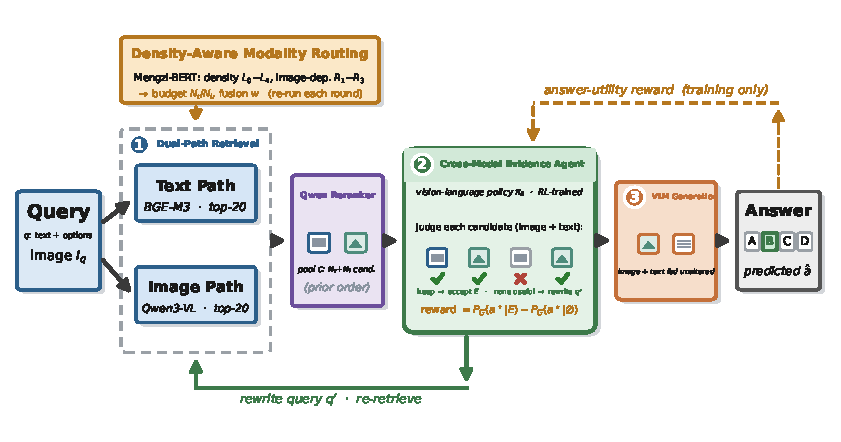
\includegraphics[width=0.95\textwidth]{fig2_architecture.pdf}}{%
    \framebox[0.95\textwidth]{\rule{0pt}{4.2cm}\ Figure~2 placeholder (system architecture)}}
  \caption{MedAlign-RAG. Dual-path retrieval feeds a density-aware router that
  allocates the text/image budget; the reranked pool is inspected by a
  vision-language agent that judges each image and text candidate and either
  accepts the evidence for generation or rewrites the query and re-retrieves
  (closing the loop). The agent is trained by reinforcement learning against an
  answer-utility reward---the lift in the frozen generator's probability of the
  correct answer. Accepted image--text evidence is passed unaltered to the
  generator.}
  \label{fig:architecture}
\end{figure*}

\subsection{Problem Formulation and Evaluation Protocol}
\label{sec:formulation}

A query is a pair $x=(q, I_q)$, where $q$ is the question text (with answer
options for multiple-choice QA) and $I_q$ is an optional query image. Given a
text corpus $\mathcal{T}$ and an image corpus $\mathcal{V}$, a retriever returns
a candidate pool $\mathcal{C}=\mathcal{C}_t\cup\mathcal{C}_i$ with
$\mathcal{C}_t\subseteq\mathcal{T}$ and $\mathcal{C}_i\subseteq\mathcal{V}$. An
agent selects an evidence set $E\subseteq\mathcal{C}$---not in one shot, but
through iterative rounds of judging, generating, or reformulating and
re-retrieving (Sec.~\ref{sec:selection})---and a vision-language generator $G$
produces the answer
\begin{equation}
  \hat{a} = G\!\left(q, I_q, E\right).
  \label{eq:generation}
\end{equation}

The distinction we stress is the \emph{form} of $E$ passed to $G$. Prior work
adopts a \emph{text-proxy} protocol in which every image evidence $e\in E$ is
replaced by its textual caption $\text{cap}(e)$, so $G$ receives text only.
We instead adopt an \emph{end-to-end image--text} protocol in which the actual
pixels of image evidence are passed to $G$. As we show empirically, the two
protocols rank methods differently: text-proxy evaluation is blind to the
quality of visual evidence and therefore misestimates reranking quality on
image-dependent queries.

\subsection{Dual-Path Retrieval}
\label{sec:retrieval}

The text path encodes $q$ with a text embedding model~\cite{chen2024bgem3} and
searches $\mathcal{T}$ by inner product, returning the top $N_t$ passages. The
image path encodes $I_q$ with the vision tower of a vision-language
model~\cite{bai2023qwenvl} and searches $\mathcal{V}$, returning the top $N_i$
images. Each candidate $c$ carries a first-stage score $s(c)$ from its own path.
The union $\mathcal{C}$, with $|\mathcal{C}|\le N_t+N_i$, forms the input to
reranking.

\subsection{Density-Aware Modality Routing}
\label{sec:routing}

The retrieval budget should follow where a query's discriminative information
lives---and, just as importantly, avoid a modality that only injects noise. A
query phrased in generic or positional terms (\emph{``which anatomical site is
shown''}) carries no discriminative textual signal; issued to the text path it
retrieves same-site, different-pathology passages that flood the pool with
homogeneous false positives. Routing must therefore be able not only to
rebalance the two paths but to \emph{suppress} one of them.

We predict two properties of $q$ with two lightweight classifiers sharing a
Chinese BERT backbone. A \emph{textual density} head outputs
$d=f_{\text{den}}(q)\in\{L_0,\dots,L_4\}$, from $L_0$ (vague, few localizable
cues) to $L_4$ (highly specific, multiple explicit constraints). An
\emph{image-dependency} head outputs $r=f_{\text{dep}}(q)\in\{R_1,R_2,R_3\}$,
from $R_1$ (text usually suffices) to $R_3$ (the image is indispensable).

Given a total budget $B=N_t+N_i$, the router allocates the image share through a
monotone function $\phi$ that increases with image dependency and decreases with
textual density,
\begin{equation}
  N_i = \big\lceil B\cdot\phi(d, r)\big\rceil,\qquad N_t = B - N_i,
  \label{eq:budget}
\end{equation}
and produces a fusion weight $w\in[0,1]$ that biases the reranker toward the
trusted modality. Routing is re-run on every retrieval round, so a query
reformulated by the agent (Sec.~\ref{sec:selection}) is re-budgeted from its new
text. Crucially, $\phi$ saturates: a
low-density, image-critical query ($L_0,R_3$) drives $N_t\!\to\!0$ and
$w\!\to\!1$, gating off the noisy text path, whereas a text-answerable query
($L_4,R_1$) drives $N_i\!\to\!0$, avoiding spurious visual matches. Unlike a
fixed fusion weight, routing can thus withdraw a modality entirely when its
signal is noise rather than evidence.

\subsection{Agentic Cross-Modal Evidence Selection}
\label{sec:selection}

Rather than take the reranker's top $K$ as final, we treat evidence selection as
a sequential decision problem solved by a vision-language agent $\pi$. The agent
sees the actual pixels of image candidates and the text of passage candidates,
judges which ones are worth keeping, and---when the pool is inadequate---rewrites
the query and retrieves again. It is trained so that the evidence it keeps
maximizes the generator's chance of answering correctly, rather than surface
relevance.

\paragraph{Initial ordering.}
The mixed pool $\mathcal{C}$ is first ordered by an off-the-shelf multimodal
reranker, using the fusion weight $w$ from routing to bias the ranking toward the
trusted modality. This ordering is only a prior; the agent, not the reranker,
decides what is used.

\paragraph{Agent policy.}
The policy $\pi_\theta$ is a small vision-language model that ingests the query
$(q,I_q)$ and the ranked candidates---image candidates as pixels, so visual
content is judged directly rather than through captions---and, at each round
$t$, emits an action $a_t$:
\begin{equation}
  a_t \sim \pi_\theta\!\left(\cdot \mid q, I_q, \mathcal{C}^{(t)}, E^{(t)}\right),
  \label{eq:policy}
\end{equation}
where $a_t$ either (i)~\emph{selects} candidates into the running evidence set
$E^{(t)}$, (ii)~\emph{accepts} $E^{(t)}$ and stops, or (iii)~\emph{rewrites} the
query to $q^{(t+1)}$, triggering a fresh retrieval round (through routing,
Sec.~\ref{sec:routing}) that refreshes the pool $\mathcal{C}^{(t+1)}$. Rewriting
gives the system a recourse absent from one-shot rerankers: a pool of
same-site, different-pathology false positives can be discarded and replaced by
a more discriminative query. The loop runs until the agent accepts or a round
budget $T$ is reached.

\paragraph{Answer-utility reward.}
The agent is rewarded by how much the accepted evidence improves the frozen
generator's confidence in the correct answer. For a multiple-choice query with
gold answer token $a^\star$, let $P_G(a^\star \mid q, I_q, E)$ be the generator's
probability of $a^\star$ given evidence $E$. The reward is the utility
\emph{lift} over answering with no evidence,
\begin{equation}
  R(E) = P_G\!\left(a^\star \mid q, I_q, E\right)
       - P_G\!\left(a^\star \mid q, I_q, \varnothing\right).
  \label{eq:reward}
\end{equation}
The second term is a per-query baseline that measures how much the generator
already knows closed-book, so the agent is credited only for evidence that
genuinely helps. Because $R$ is read from the generator's answer distribution, it
needs \emph{no passage-level relevance labels}---the multiple-choice answer is
the only supervision. Evidence that is topically related but useless yields no
lift, and confidently-wrong homogeneous-image matches, which pull probability
toward a distractor, are penalized---directly targeting~(P2).

\paragraph{Training.}
We optimize $\theta$ with policy-gradient reinforcement learning, maximizing the
expected reward $\mathbb{E}_{a_{1:T}\sim\pi_\theta}\!\left[R(E)\right]$ over
sampled trajectories, with the generator $G$ frozen throughout so the reward
reflects evidence quality alone. Because the reward is defined on the end-to-end
image--text answer distribution, training \emph{requires} the corrected
evaluation protocol (Sec.~\ref{sec:formulation}): under a text-proxy protocol the
generator never sees image evidence, and the utility signal that drives learning
would be blind to it.

\subsection{Multimodal Generation}
\label{sec:generation}

The selected set $E$---original image pixels together with text passages---is
provided to the vision-language generator following Eq.~\ref{eq:generation}. No
image is replaced by a caption, so visual evidence contributes directly to the
answer.

\section{Experiments}
\label{sec:experiments}

\subsection{Setup}
\label{sec:setup}
We evaluate on EndoBench~\cite{endobench}, a multiple-choice endoscopic QA
benchmark of $6{,}832$ questions, of which $84.5\%$ are image-only, $15.3\%$
image--text, and $0.1\%$ text-only. The text corpus and image corpus are indexed
separately; dual-path retrieval returns the top candidates from each path, which
routing re-budgets per query and an off-the-shelf multimodal reranker orders. The
agent policy is a small vision-language model; the generator is a frozen
vision-language model that receives image--text evidence directly. The agent is
trained by policy-gradient reinforcement learning against the answer-utility
reward (Eq.~\ref{eq:reward}) with the generator frozen, using only the
benchmark's multiple-choice answers as supervision. We report multiple-choice
accuracy overall and split by image-only vs.\ image--text queries.
% Implementation details anonymized for submission.

\subsection{Evaluation Blindness: Text-Proxy vs.\ Image--Text Input}
\label{sec:blindspot}
We first quantify the evaluation blind spot (C3): holding the retrieved evidence
fixed, we compare feeding the generator textual captions of image evidence
(text-proxy) against feeding the actual pixels (image--text). The gap, largest on
image-dependent queries, measures how much visual evidence a text-proxy protocol
hides. This experiment does not depend on the agent and can be run now
(Table~\ref{tab:blindspot}).

\begin{table}[t]
  \centering
  \begin{tabular}{lccc}
    \toprule
    Input to generator & Image-only & Image--text & Overall \\
    \midrule
    Text-proxy (captions) & -- & -- & -- \\
    Image--text (pixels)  & -- & -- & -- \\
    \bottomrule
  \end{tabular}
  \caption{Evaluation blindness (C3): accuracy under text-proxy vs.\ end-to-end
  image--text input, evidence held fixed. \emph{TBD.}}
  \label{tab:blindspot}
\end{table}

\subsection{Main Results}
\label{sec:main}
Table~\ref{tab:main} compares MedAlign-RAG against no-retrieval (closed-book),
top-$K$ retrieval, a cross-encoder reranker~\cite{nogueira2019passage}, a
graph-based reranker, and agentic-RAG baselines adapted to the multimodal
setting~\cite{asai2024selfrag,jin2025searchr1,shao2023iterretgen}, all under the
corrected image--text protocol. \emph{Results TBD.}

\begin{table*}[t]
  \centering
  \begin{tabular}{lccc}
    \toprule
    Method & Image-only & Image--text & Overall \\
    \midrule
    No retrieval (closed-book)       & -- & -- & -- \\
    Top-$K$ retrieval                & -- & -- & -- \\
    Cross-encoder rerank~\cite{nogueira2019passage} & -- & -- & -- \\
    Graph-based rerank               & -- & -- & -- \\
    Self-RAG (multimodal)~\cite{asai2024selfrag}    & -- & -- & -- \\
    Search-R1 (multimodal)~\cite{jin2025searchr1}   & -- & -- & -- \\
    Iter-RetGen (multimodal)~\cite{shao2023iterretgen} & -- & -- & -- \\
    \midrule
    MedAlign-RAG (ours)              & -- & -- & -- \\
    \bottomrule
  \end{tabular}
  \caption{Main results on EndoBench under the corrected image--text protocol.
  \emph{TBD.}}
  \label{tab:main}
\end{table*}

\subsection{Ablation Study}
\label{sec:ablation}
We ablate the agent's components: (i)~value judgment on/off (accept the
reranker's top $K$ vs.\ let the agent select); (ii)~query rewriting and
re-retrieval on/off; (iii)~reward design (answer-utility lift vs.\ a
relevance/format reward); (iv)~maximum round budget $T$; and (v)~density-aware
routing on/off. \emph{Results TBD.}

\subsection{Analysis}
\label{sec:analysis}
We present case studies including a visual-similarity false positive that
similarity-based selection accepts but the agent rejects, and a query the agent
rewrites to recover from a poor initial pool; plus the distribution of rounds
used and of selected-evidence modality across query types. \emph{Results TBD.}

\section{Conclusion}
\label{sec:conclusion}

We revisited evidence selection in multimodal medical RAG and argued that the
prevailing recipe---score candidates for relevance and take the top $K$ in a
single pass---is fundamentally passive: it conflates relevance with
answer-utility, offers no recourse when the retrieved pool is inadequate, and,
on visually homogeneous medical images, systematically admits high-confidence
but clinically wrong evidence. We recast selection as an \emph{agentic search}
process. A vision-language agent judges image and text candidates cross-modally
and either accepts them for generation or rewrites the query to re-retrieve,
trained with an \emph{answer-utility reward}---the lift in a frozen generator's
probability of the correct answer---which needs only multiple-choice supervision
and no passage-level labels. A density-aware router allocates the retrieval
budget on every round and can suppress a modality whose signal is noise, and we
evaluate under a corrected end-to-end image--text protocol that feeds the
retrieved images to the generator directly.

Our framework has limits. The reward is a per-query answer-probability lift, so
it presumes access to gold answers at training time and is most natural for
multiple-choice supervision; extending answer-utility rewards to open-ended
medical generation, and reducing the cost of iterative re-retrieval, are natural
next steps. More broadly, we hope answer-utility--driven, cross-modal agentic
retrieval proves useful beyond endoscopy---wherever visual similarity is a poor
proxy for the evidence a model actually needs.


\bibliography{references}

\end{document}
